\section{DRAM Device Architecture}\label{sec:dram-arch}

The organization of a typical DRAM device is shown in
figure~\ref{fig:dram-device}. It has three core main:
\emph{address}, divided into bank-address (BA) and (intra-bank) address (A);
\emph{command}, which include clock enable (CKE, CKE\#) and a collection of other
signals (CAS\#, RAS\#, WE\#, CS\#) which encode different DRAM instructions or
\emph{commands}; and \emph{data}, which includes data payload (DQ), data
strobes (DQS), and write-data masks (DM).

Within a DRAM device, arrays of \emph{bit cells} are hierarchically arranged into multiple parallel
\emph{banks}.  Banks provide the primitive level of concurrency in a DRAM
memory system. They can service independent requests, assuming they do not
simultaneously require shared resources like the data bus.

\begin{figure}
	\centering
	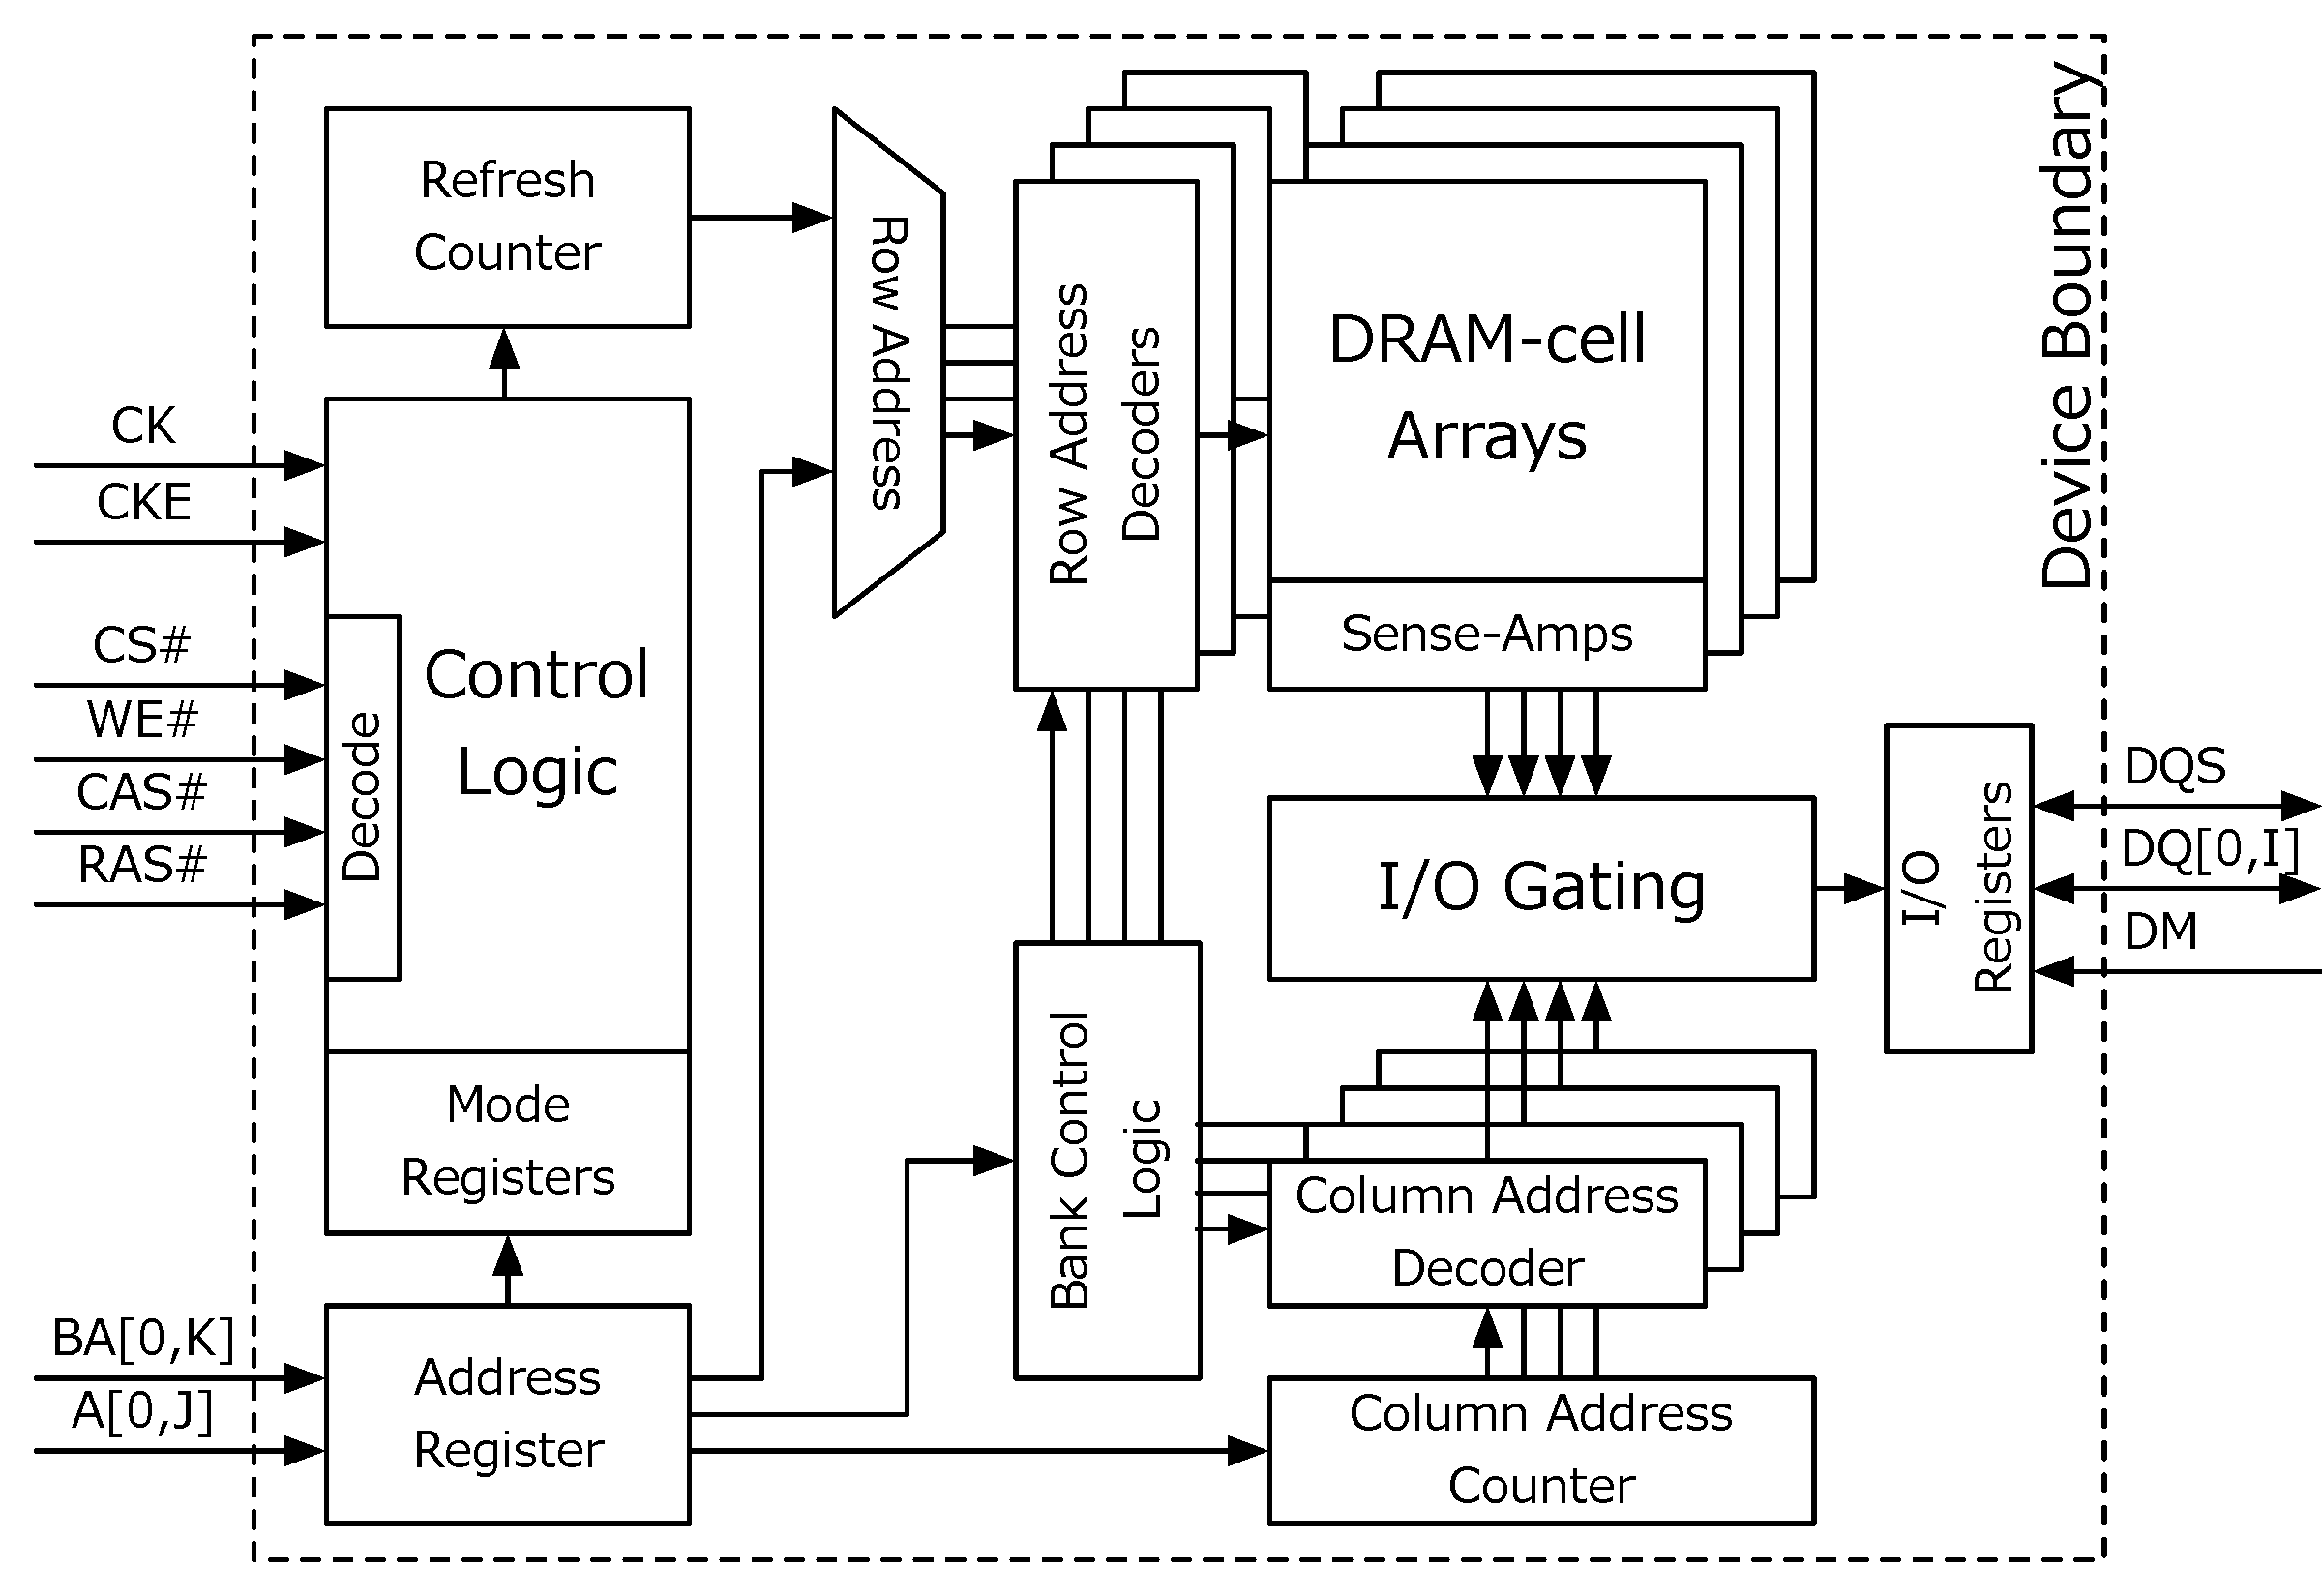
\includegraphics[width=16cm]{figures/dram-device.pdf}
    \caption{The organization of a typical DRAM device.}
	\label{fig:dram-device}
\end{figure}

A basic DRAM operation requires a series of three commands: \emph{activate
(ACT)}, \emph{column access~(CAS)}, and \emph{precharge~(PRE)}. Initially, the
bitlines of the DRAM-cell array are precharged to VDD/2, and DRAM cells are
isolated from the bitline by a single access transistor. To a commence a read or write, first, a row must be
\emph{opened}. The ACT command achieves this by enabling the wordline of the
array corresponding to a single \emph{row} of the bank. In what is called the \emph{sense}
phase, charge sharing between the cells of the now-open row and the bitlines of
the array create perturbations in the bitline voltages that are detected an
array of differential sense-amplifiers. This is temporarily destructive: the
bit cell voltages are driven to approximately VDD/2. However, after the
sense phase, the amps restore the cell voltage by driving the bitline back
towards VDD or GND based on the detected state of the bit cell. The sense-amps
also act as a \emph{row buffer}, which saves the sensed state until it is
instructed to close -- more on this shortly.

A CAS command then selects a subset of the row buffer to read or write~(CASR
and CASW commands respectively). In double-data rate~(DDR) SDRAM, data is
bursted over successive rising and falling edges of the data strobe. While the
row remains open, successive reads or successive writes can be made by issuing
new CAS commands without any data-bus bubbles\footnote{There is a penalty for
interleaving reads and writes as ownership of the data bus must be transferred
between the device and controller.~(See $t_{WTR}$ in
table~\ref{tbl:dram-timings}.)}

Finally, to access a row not stored in the buffer, a PRE command must be issued
to \emph{close} the row. This disables the wordline, which isolates the
restored bit cells and enables the bitline to be precharged back to VDD/2 to
prepare for a new access.

DRAM is named dynamic RAM because it gradually loses its stored state over time
as bit cell capacitors leak. DRAM-cell retention rates vary on-die and between
dies and are highly sensitive to temperature~(warmer cells leak faster). To
maintain their state, DRAM cells must be periodically ``refreshed"; activating
a row of cells is sufficient to refresh them. As part of the DRAM standards,
JEDEC mandates that cells must be refreshed on-average once every 64 ms, an
interval they have maintained from DDR through DDR4. Since activations to every
row cannot generally be guaranteed during normal use, DRAM devices are
refreshed explicitly with a refresh command~(REF). To reduce complexity, this
command refreshes a constant number of contiguous in all banks concurrently, beginning at the row
address indicated by the refresh counter. DRAM
manufacturers generally have kept the number of refresh commands required to
iterate through the entire array constant in all banks concurrently: 8192 commands per 64 ms interval, or
one every 7.8 $\mu s$.  As a result, refresh commands take longer to execute on
devices with more rows per bank.

At the system level, multiple DRAM devicess can be arranged in parallel to widen the
data bus; address and command buses fan out to each device. For more concurrency,
and to support larger memory capacities, multiple \emph{ranks} of DRAM devices
may be used.  Here, generally, the command and data buses are shared between
all ranks, with a one-hot chip-select (CS\#) indicating which rank a command is
addressing.

Since logic is expensive in a conventional DRAM-process technology, it is
minimized. DRAM commands must scheduled in accordance to part-specific timings
if the devices are to function correctly. We give a list of key timings in a DDR
protocol in table~\ref{tbl:dram-timings}. These have been taken, with
some modification, from \textit{Memory Systems: Cache, DRAM,
Disk}\cite{drambook}.

\begin{table}[htb]
\begin{center}
\resizebox{\textwidth}{!}{%
    \begin{tabular}{|p{0.20\textwidth}|p{0.8\textwidth}|}
    \hline
    \textbf{Name} & \textbf{Description} \\
    \hline
    \hline
    \textbf{$t_{AL}$} & Additive Latency. Additional latency added to column access commands. \\
    \textbf{$t_{CAS}$~($t_{CL}$)} & Column Access Strobe latency. Delay between
    when a CASR command is received and when the first beat of read data is
    returned. \\ \textbf{$t_{CCD}$} & Column-to-Column Delay. Minimum duration
    between two consecutive column commands. \\ \textbf{$t_{CMD}$} & Command
    transport duration. The duration a command occupies the command bus. \\
    \textbf{$t_{CWD}$~($t_{WL}$)} & Column Write Delay. The delay between a
    CASW command and the when the controller must present the first beat of
    write data. \\
    \textbf{$t_{FAW}$} & Four row Activation Delay. A rolling time window
    during which only four ACT commands may be made to a rank of a DRAM
    devices.\\
    \textbf{$t_{RAS}$} & Row Access Strobe. The minimum duration after an ACT
    command during which the row must be kept open before issuing a PRE command
    to close it. \\
    \textbf{$t_{RC}$} & Row Cycle time. The minimum duration required
    to open, and close a row. $t_{RC} = t_{RAS} + t_{RP}$ \\
    \textbf{$t_{REFI}$} & Refresh Interval. The average period of time between refresh commands. \\
    \textbf{$t_{RCD}$} & Row-to-Column Delay. The minimum duration after an
    ACT command that CAS commands may be issued to the newly-opened row.  \\
    \textbf{$t_{RFC}$} & ReFresh Cycle time. The minimum duration after a refresh
    command that activation commands may be issued. \\
    \textbf{$t_{RP}$} & Row Precharge delay. The minimum duration after a
    precharge command that an ACT to the same bank may be issued. \\
    \textbf{$t_{RRD}$} & Row-to-Row Delay. The minimum duration between ACT commands to the same rank. \\
    \textbf{$t_{RTP}$} & Read-To-Precharge delay. The mimimum duration after a CASR command that a PRE command may be issued to the same row. \\
    \textbf{$t_{RTRS}$} & Rank-To-Rank Switching delay. Accounts for time to change termination schemes on DQ and DQS buses when switching between ranks. \\
    \textbf{$t_{WR}$} & Write Recovery time. The minimum duration after a CASW command that a PRE command may be issued to the same row. \\
    \textbf{$t_{WTR}$} & Write TurnaRound Time. The minimum duration after a CASW command that a CASR may be issued to the same row. \\
    \hline
\end{tabular}}
\end{center}
\caption{A list of key timings for a conventional DDRx SDRAM}
\label{tbl:dram-timings}
\end{table}%

\clearpage
\section{DRAM Controller Architecture}

A DRAM controller is responsible for responding to memory
requests from one or more requestors by scheduling those requests over its
attached memories as a judicious stream of DRAM commands.

Memory access scheduling~(MAS) is the process by which, for a given cycle, a
controller selects a single DRAM command to be issued from a legal set. Legal
commands are constrained by the current state of each bank, the availability of
shared resources like the command and data buses, and the timing constraints
imposed by the DRAM devices. Good MAS policies strike a delicate balance
between minimizing latency, maximizing bandwidth, minimizing power, and
maintaining quality-of-service guarantees across multiple threads of execution.
There are plethora of academic papers on MAS policies, and still more
industrial patents on the subject. In this report we consider two popular MAS
policies: first-come first-serve, and first-ready, first-come first-serve.

\subsection{First-Come First-Serve~(FCFS) Policy}\label{sec:fcfs} Commands for the
oldest pending memory reference are issued first. This is the simplest MAS
policy, but tends to under-utilize available DRAM bandwidth as younger requests
that may hit in the row-buffer are not issued before older commands that miss.
FCFS schedulers are common in older machines, and those that present few
concurrent memory requests.

\subsection{First-Ready FCFS~(FR-FCFS)~\cite{frfcfs} Policy}\label{sec:frfcfs}
First, ready~(legally issuable) column commands are prioritized over ready row
commands. Second, commands for older references are prioritized over younger
ones. This permits younger but ready column commands to be issued before older
row commands. FR-FCFS is a relatively simple scheme that improves bandwidth
utilization considerably. It is the de facto standard against which new MAS
policies for machines with a single stream of memory references~(like
single-core out-of-order machines), are compared.

\section{Power Consumption in DRAM Memories}\label{sec:dram-power}

DRAM power consumption can be divided into six different classes: activation
(including precharge), read, write, termination, refresh, and background power.

Activation is generally the largest component of DRAM power consumption.  In an
effort to maximize areal density and reduce cost-per-bit, DRAM sub-arrays have
long, high capacitance bitlines, which are driven to VDD or ground during the
restore phase of an activation. Moreover, DRAM rows are long: thousands of
bitlines are simultaenously charged or discharged in a single activation. These
two properties lead to high peak-current draw during an activation. In order to
stay within a power envelope where DRAM devices can be cooled passively without
heatsinks, DRAM manufacturers put limits on activation frequency through
$t_{RRD}$ and $t_{FAW}$ constraints (see table\ref{tbl:dram-timings}).

Read and write power consumption accounts for the power dissipated as data is
driven between the I/Os of the chip and its various sub-arrays, as well as the
power used to decode the read or write command.

Refresh power accounts for the power lost during the successive activations and
precharges of a refresh command. It is a growing component of power consumption
as modern DRAM devices trend towards higher row counts. Higher row counts impose
that more rows must be refreshed per command which forces the device to spend
more time in refresh (higher $t_{RFC}$).

Termination power accounts for the power dissipated in on-die termination
resistors of a device during a write, and by the output buffers of a device
during a read. In multi-rank systems, this also includes power dissipated in
the termination resistors of ranks not being addressed.

Finally, background power accounts for leakage of various circuits within the
IC. Here there are two dimensions of note. First, activated banks
leak more than precharged banks. Second, powered-down ranks~(CKE low) leak less
than powered-up ranks~(CKE high).


\section{Simulation of DRAM-based Memory Systems}

The current state of the art in DRAM simulation in academia are cycle-accurate
software simulators like DRAMSim2~\cite{dramsim}, Ramulator~\cite{ramulator} and
USIMM~\cite{usimm}. These simulators generate DRAM command streams that have been
validated against industrial models~(for some standards). Both Ramulator and
DRAMSim2 can be easily integrated into Gem5~\cite{gem5}, though Gem5 includes a
detailed event-based model of its own~\cite{gem5event}. In trace-driven mode,
operating at full throughput and only as a timing-model, these cycle-accurate
models simulate at frequencies ranging from hundreds of KHz to ones of
MHz~\cite{ramulator}.

In order to model power, Micron has described a strategy~\cite{micronpower}
that assigns an average current draw to the modes of power dissipation
described in section~\ref{sec:dram-power}. Micron has also provided
spreadsheets that generate estimates based on system-level measurements of DRAM
activity, including proportion of the time the devices spend read and writing,
and the row-buffer hit rate.  Conversely, DRAMSim2 directly implements the
strategy by integrating the approriate current based on the state of the
simulated memories.

One limitation of the Micron approach, is that it does not account for the
power dissipation of the controller itself. However, for modest memory
controller implementations, this should be small.
